\documentclass[krantz1,ChapterTOCs]{krantz}
\usepackage{amssymb}
\usepackage{amsmath}
\usepackage{graphicx}
\usepackage{subfigure}
\usepackage{makeidx}
\usepackage{multicol}
\usepackage{mathptmx}
\usepackage{newtxtext,newtxmath}
%\usepackage{hyperref}
\usepackage{lipsum}


\frenchspacing
\tolerance=5000

\makeindex
\begin{document}
\newtheorem{theorem}{Theorem}
\newtheorem{exercise}{Exercise}[chapter]
\newtheorem{example}{Example}
\newtheorem{definition}{Definition}
\newtheorem{proof}{Proof}


\frontmatter

\title{AI and Sustainability for Emerging Markets}
\author{Dinesh Verma}
\maketitle


%%%Placeholder for front matter

%\halftitle

%\booktitle

%\locpage

\cleardoublepage
\thispagestyle{empty}
\vspace*{\stretch{1}}
\begin{center}
\Large\itshape
To the Enterprise NeuroSystem Group\\
and the employers of the contributors \\
who have supported our involvement \\
in this open-source project.
\end{center}
\vspace{\stretch{2}}
%\cleardoublepage
\setcounter{page}{7} %previous pages will be reserved for frontmatter to be added in later.
\tableofcontents
\chapter*{Foreword}

Aboritiorior maio. Optaess inullore cum autate niate nonem ut ario. Ut labor soloreped magniae ipsum etur sunt magnatiorpos nonsequi ut aliquideles quam quisque magnatia voluptae poreperiat.
Ibus, num escilla boreribus, utem qui arum fugitae rrorit que ide volum debit faci conseque nus as quo doluptatur autem qui odis dero esequis nihillaborio di audit ut moluptate opta dolorere vellabore verum fugita del molori occus pores est et fugiati audis enimus sitentur?
Possequ asperupita sedit, int.
Im dolo vid quo te quis dollam re ne que sime parchit aspici unto te accusam eium eium reptas sitatio etur?
Gent pereperum endunt magnate pa dolore cuptatent dolum aliquae eturera voluptat vent odiatinusaes quos aliquias minvel ipsunt adicid eossunto tet es ex estios sit volupta commo tendemp oribus, aut in nimped quam utate suntiam enis eictatem doluptatem volorendis archilibus.
Ucipsan dissimp eriatio dis qui aspe ium et anda consequis min rest, vit ad que liqui asitatur, nonsed moles dolorum illacienis adit quias in eiciet doluptasint doluptisque volupta senihillaut amus ut et es undic tem velit estrunt et pra quaerchit ut opti rero ipis modio tendae prorat ea velit ut es es coruptatur molent explabo ruptat labo. Et aut quos que dolut velibuscil maxim debite exces moluptatium volupiendam nullignatus.
Qui omnit pla ium qui alicim repe vendi delenim intur, quia volorum, esti te pa cusam que simi, tem et, eosam, conecae nim vent.
Ficidebit fugitatis reptat lant.
Mos voluptas sit officiminci bea et inci que estrunt maximet a peliqui aspeliquos et aperior re saperum rerchicia quideri volorro quia veliquam faceris ma voloreptati qui omnis mod mo tem repediciis rem. Et quias molorit imillam ne pra ipsam id moles min nonsequos exerum volest et, temporepudae sunt rem nobit modi dolorepta volenim dolupti beatiberum ipsuntenis ditenis evellaut omnima volorit eosamet fugiati volorro blaborem quis acessunt.

Um con commolupta si conecto rporum dolliqui ut odit ut prem. Inihit erorior eptur, sitaten esequi atiaestis que vel ium quosae prerunt issimus mi, aborat ium voluptasin nulpa quam lique pro dus imil est liaturi onseque num am, site num eatecto taquid magnim alitiun diciaspit volor aspe nimagnis anis autati quoditis que volupta tiant, eatio. Et utet et volupta turiorum facillabo. Elique pore etur sit explant atibusciet adit venimuscimus voluptibusa pro et et estia venditiumqui nonessitist, sim ad qui int, que eatiorent ipsant landior maximet, tempore mpedis aciuntio tem sunt reped etur?
Ugit, aut la et ese pligendebis si quam quam nonsequ atquodio con nemporrorero mil illestiatet apic tet qui conectia vollab ipiciis et il es dolupta quaspedis quo et rerunt inum et ea delenih ilistempero beri culpa doluptur, el maximenimus modias as di del ima con repuda vita eat iduntis magnatent enda voluptassin re es molorecerum quissit lab ipsanda eptate samus et qui utatem eatium faces adictur? 

Ficate et et quam laccatinum et a sinverepe core cum quat.
Fugiam name commos volupta tiusantus voluptatium rerum reius consendi des aut la doluptate si que sunt aut odi comnia parunt voluptatur, aut ressitiore et aut liberit atibusdae cuptati nctotas dendebit et isquaspiento doluptatia nonet ad quo omnisit ibusam, volorib usamus.
Da quam fugiatem volupta quaessequodi ni tem quia vit idundende est, imo quis que am lam nos molorep ellenienis dolorecusdae re nossus autenditi derchicius nates sum haritate liaturit, ulliquam cum, susa corepudam harum eaquodicimin corenducit, sit, coreperro moloreperem eventem. Ignation nonsequias moluptam quias modia et, tem. Ut erupti doluptatem volorro corerum quae plabore mporrum fugias arum laborionsed maximod et hilia autas aspis aut ipsum rest earchilis enecero tem res desere con restemporem faceped ma dolupta sperore mperectem. Nempelenim nullore corest, quatus aut maximus quunt illaboremped quidio voluptatur?

Ati volorepudist laborrum nam, commolecto il ius.
Eni omnit labor maxim dolores as as sit as et libusapis veliqui busciae quam estius, conemporibus ant ut as consedi gendaerum volum non nossunt eum doles im quibus de pe non rem vendit, sunt autem eiusam dolupta dia delleseque iunders pellamus.
Cones quias que oditaec tessitaepe rem ent es moluptatius.
Aximinus ipsae si alibus.
Onsed magnimuscit rercid maionsed que nosaerum re et ellupti busant anim quide iur atust as atqui offic tet ut odicimus ea pratia deribustio. Tection sernatis dolo magnat lamusdae sunt.
Otat labo. Ut que sit latque ped moluptio ea doloressed eatusaperiam eosse nonsequi aces suntur rempore mporepe dition preheni magnihi ligendant faccus.


\chapter*{Preface}

Quantum networks and quantum computing have created a significant amount of excitement and interest in the technical community. As with any emerging technology, there is a lot of potential opportunity in the exploitation of that technology, but frequently the implications of the technology are over-inflated and difficult to pinpoint. A significant amount of confusion also arises due to the high degree of specialization that exists in the present technical community, making it difficult to assess and evaluate the benefits of new technology. 

There are many books existing on quantum networks, but most of them are geared towards the physicists and theoreticians working on improving the quantum communication technologies. That leaves many software professionals and computer scientists wondering about the implications of these networks, and what impact they may have on the future of information technology. 

This book attempts to bridge that gap that exists, providing an overview of the quantum networks from the perspective of a software user. It discusses the current state of quantum networks, how it compares to the traditional computer networks, and what type of software applications would benefit from the use of quantum networks. 

We hope the simplified approach to deal with quantum networking technologies in this book will be useful to the software engineer, as well as the CTOs and CIOs in many enterprises as they try to assess the impact of quantum technologies on their businesses. 

\listoffigures
\listoftables
%%\twocolumn
\chapter*{Contributors}

\begin{multicols}{2}
\contributor{Abhay Ratnaparkhi}{IBM}{Armonk, New York, U.S.A.}

\contributor{Sheeba Prakash}{IBM}{Armonk, New York, U.S.A.}

\contributor{Anindita Das}{IBM}{Armonk, New York, U.S.A.}

\contributor{Mathews Thomas}{IBM}{Armonk, New York, U.S.A.}

\contributor{Dinesh Verma}{IBM}{Armonk, New York, U.S.A.}

\contributor{Sourav Mazumder}{IBM}{Armonk, New York, U.S.A.}

\contributor{Bill Wright}{Red Hat}{Raleigh, North Carolina, U.S.A.}

\contributor{Sanjay Aiyagari}{Red Hat}{Raleigh, North Carolina, U.S.A.}

\contributor{Josh Purcell}{Red Panda}{San Francisco, California, U.S.A.}

\contributor{John Overton}{Kove}{Chicago, Illinois, U.S.A.}

\contributor{Amdy Poling}{Kove}{Chicago, Illinois, U.S.A.}

\end{multicols}
%\thispagestyle{empty}
\begin{symbollist}{000000}
\symbolentry{$\alpha$}{To solve the generator maintenance scheduling, in the  past, several mathematical techniques have  been applied.}
\symbolentry{$\sigma^2$}{These include integer programming, integer linear programming, dynamic programming, branch and bound etc.}
\symbolentry{$\sum$}{Several heuristic search algorithms have also been developed. In recent years expert systems,}
\symbolentry{$abc$}{fuzzy approaches, simulated annealing and genetic algorithms have also been tested.}
\symbolentry{$\theta\sqrt{abc}$}{This paper presents a survey of the literature}
\symbolentry{$\zeta$}{ over the past fifteen years in the generator}
\symbolentry{$\partial$}{maintenance scheduling. The objective is to}
\symbolentry{sdf}{present a clear picture of the available recent literature}
\symbolentry{ewq}{of the problem, the constraints and the other aspects of}
\symbolentry{bvcn}{the generator maintenance schedule.}
\end{symbollist}

\mainmatter

\part{Introduction}
%
%
% Important -- Do not update this chapter of subdirectories. 
% This is meant as an example so we can see how to incorporate the various commands in the chapter
% This acts like samples for figures, tables, call-out text etc. 

\chapterauthor{Author Name1}{Affiliation text1}
\chapterauthor{Author Name2}{Affiliation text2}
\chapterauthor{Author Name3}{Affiliation text3}
\chapterauthor{Author Name4}{Affiliation text4}
\chapter{Modeling Topics for Detection and Tracking}
\label{chap:chapter_model}

This is an introductory section. 

\section{Introduction}\label{intro}
The term reliability usually refers to the probability that a
component or system will operate satisfactorily either at any particular  
instant at which it is required or for a certain length of
time. 

Fundamental to quantifying reliability s a knowledge of how to
define, assess and combine probabilities \cite{Bontempi2005Adaptive}. This may hinge on identifying the
form of the variability which is nherent n most processes. If all
components had a fixed known lifetime there would be no need to model
reliability.

A component part for an electronic item is
manufactured at one of three different factories, and then delivered to
the main assembly line.Of the total number supplied, factory A supplies
50\%, factory B 30\%, and factory C 20\%. Of the components
manufactured at factory A, 1\% are faulty and the corresponding
proportions for factories B and C are 4\% and 2\% respectively. A
component is picked at random from the assembly line. What is the
probability that it is faulty? 

\begin{VF}
``A Process is a structured, measured set of activities designed to produce a specific output for a particular customer
or market---A process is thus a specific ordering of work activities across time and space, with a beginning, an end.
and clearly defined inputs and outputs: a structure for action.''

\VA{Thomas Davenport}{Senior Adjutant to the Junior Marketing VP}
\end{VF}

\begin{table}[b!]
%\noautomaticrules
\tabletitle{Now we are engaged $(a_g^a)$ $\big(a_g^a\big)$ in a great civil war, testing whether that
nation, or any nation so conceived.}%
\begin{tabular}{lccc}
\tch{Scene}    &\tch{Reg. fts.} &\tch{Hor. fts.} &\tch{Ver. fts.}\\
Ball &19, 221 &4, 598   &3, 200\\
Pepsi$^a$&46, 281 &6, 898 &5, 400\\
Keybrd$^b$   &27, 290 &2, 968 &3, 405\\
Pepsi    &14, 796 &9, 188 &3, 209\\
\end{tabular}
\end{table}


\subsection{A component part}
A component part for an electronic item is
manufactured at one of three different factories, and then delivered to
the main assembly line.Of the total number supplied, factory A supplies
50\%, factory B 30\%, and factory C 20\%. Of the components
manufactured at factory A, 1\% are faulty and the corresponding
proportions for factories B and C are 4\% and 2\% respectively. A
component is picked at random from the assembly line. What is the
probability that it is faulty \cite{ilyas2004hsn}? 
A component part for an electronic item is
manufactured at one of three different factories, and then delivered to
the main assembly line.Of the total number supplied, factory A supplies
50\%, factory B 30\%, and factory C 20\%. Of the components
manufactured at factory A, 1\% are faulty and the corresponding
proportions for factories B and C are 4\% and 2\% respectively. A
component is picked at random from the assembly line. What is the
probability that it is faulty? 
A component part for an electronic item is
manufactured at one of three different factories, and then delivered to
the main assembly line.Of the total number supplied, factory A supplies
50\%, factory B 30\%, and factory C 20\%. Of the components
manufactured at factory A, 1\% are faulty and the corresponding
proportions for factories B and C are 4\% and 2\% respectively. A
component is picked at random from the assembly line. What is the
probability that it is faulty? 



\paragraph{MultiRelational $k$-Anonymity.} Most works on $k$-anonymity focus on anonymizing a single data table; however, a real-life \cite{diamantaras1996pcn} database usually contains multiple relational tables. This has proposed a privacy model called \emph{MultiR $k$-anonymity} to ensure $k$-anonymity on multiple relational tables. Their model assumes that a relational database contains a person-specific table $PT$ and a set of tables $T_1,\cdots,T_n$, where $PT$ contains a person identifier $Pid$ and some sensitive attributes, and $T_i$, for $1 \leq i \leq n$, contains some foreign keys, some attributes in $QID$, and sensitive attributes. The general privacy notion is to ensure that for each record owner $o$ contained in the join of all tables $PT \Join T_1 \Join \cdots \Join T_n$, there exists at least $k-1$ other record owners share the same $QID$ with $o$. It is important to emphasize that the $k$-anonymization is applied at the \emph{record owner} level, not at the \emph{record} level in traditional $k$-anonymity. This idea is similar to $(X,Y)$-anonymity, where $X=QID$ and $Y=\{Pid\}$.
\begin{extract}
A component part for an electronic item is \cite{hyvarinen2001ica}
manufactured at one of three different factories, and then delivered to
the main assembly line.Of the total number supplied, factory A supplies
50\%, factory B 30\%, and factory C 20\%. Of the components
manufactured at factory A, 1\% are faulty and the corresponding
proportions for factories B and C are 4\% and 2\% respectively. 
\end{extract}
A component part for an electronic item is
manufactured at one of three different factories, and then delivered to
the main assembly line.Of the total number supplied, factory A supplies
50\%, factory B 30\%, and factory C 20\%. Of the components
manufactured at factory A, 1\% are faulty and the corresponding
proportions for factories B and C are 4\% and 2\% respectively. A
component is picked at random from the assembly line. What is the
probability? 

\begin{shadebox}
A component part for an electronic item is
manufactured at one of three different factories, and then delivered to
the main assembly line.Of the total number supplied, factory A supplies
50\%, factory B 30\%, and factory C 20\%. Of the components
manufactured at factory A, 1\% are faulty and the corresponding
proportions for factories B and C are 4\% and 2\% respectively. A
component is picked at random from the assembly line. What is the
probability that it is faulty? 
\end{shadebox}

In most literature on PPDP, they \cite{jolliffe2002pca} consider a more relaxed, yet more practical, notion of privacy protection by assuming limited attacker's background knowledge. Below, the term ``victim" refers to the record owner being linked. We can broadly classify linking models to two families.

\begin{example}
One family considers a privacy threat occurs when an attacker is able to link a record owner to a record in a published data table, to a sensitive attribute in a published data table, or to the published data table itself. We call them \emph{record linkage}, \emph{attribute linkage}, and \emph{table linkage}, respectively. In all types of linkages, we assume that the attacker knows the $QID$ of the victim. 
\end{example}

In record and attribute linkages, we further assume that the attacker knows the presence of the victim's record in the released table, and seeks to identify the victim's record and/or sensitive information from the table \cite{yao2002can}. In table linkage, the attack seeks to determine the present or absent of the victim's record in the released table. A data table is considered to privacy preserved if the table can effectively prevent the attacker from successfully performing these types of linkages on the table \cite{madden2002tta}. Sections~\ref{intro}-\ref{sec:reclinkage} study this family of privacy models.
\begin{equation}
\mbox{var}\widehat{\Delta\Omega\Gamma} = \sum_{j = 1}^t \sum_{k = j+1}^t
\mbox{var}\,(\hat{\alpha}_j - \hat{\alpha}_k)  = \sum_{j = 1}^t
\sum_{k = j+1}^t \sigma^2(1/n_j + 1/n_k). \label{2delvart2}
\end{equation}


An obvious measure of imbalance is just the difference in the
number of times the two treatments are allocated
\begin{equation}
D_n = |n_A - n_B|. \label{2deffD}
\end{equation}
For rules such as deterministic allocation, for which the expected
value of this difference can be calculated, we obtain the population
value ${\cal D}_n$.

\begin{shortbox}
\Boxhead{Box Title Here}
Another family aims at achieving the \emph{uninformative principle}: The published table should provide the attacker with little additional information beyond the background knowledge. There should not be a large difference between the prior and posterior beliefs; otherwise, there is a privacy threat~\cite{jain2004ass, jolliffe2002pca}. Many privacy models in this family are designed for statistical database and do not distinguish attributes in $T$ into $QID$, but some of them could also thwart record, attribute, and table linkages. Section~\ref{intro} studies this family of privacy models.

Let $m$ be a prime number. With the addition and multiplication as 
defined above, $Z_m$ is a field.
\end{shortbox}

Another family aims at achieving the \emph{uninformative principle}: The published table should provide the attacker with little additional information beyond the background knowledge. There should not be a large difference between the prior and posterior beliefs; otherwise, there is a privacy threat~\cite{jain2004ass, jolliffe2002pca}. Many privacy models in this family are designed for statistical database and do not distinguish attributes in $T$ into $QID$, but some of them could also thwart record, attribute, and table linkages. Section~\ref{intro} studies this family of privacy models.

\begin{theorem}\label{1th:Z_m}
Let $m$ be a prime number. With the addition and multiplication as 
defined above, $Z_m$ is a field.
\end{theorem}


\section{Record Linkage Model}\label{sec:reclinkage}

In the privacy attack of \emph{record linkage}, some value $qid$ on $QID$ identifies a small number of records in the released table $T$,
called a \emph{group}. If the victim's $QID$ matches the value
$qid$, the victim is vulnerable to being linked to the small
number of records in the group \cite{madden2005taq}. In this case, the attacker faces
only a small number of possibilities for the victim's record, and
with the help of additional knowledge, there is a chance that the
attacker could uniquely identify the victim's record from the
group.


\begin{table}
\tabcolsep10pt
    \tabletitle{Examples for illustrating attacks}
    \begin{tabular}{|c|c|c|c|}
        \hline
        \textbf{Job} & \textbf{Sex} & \textbf{Age} & \textbf{Disease} \\
        \hline
        Engineer & Male & 35 & Hepatitis \\
        Engineer & Male & 38 & Hepatitis \\
        Lawyer & Male & 38 & HIV \\
        Writer & Female & 30 & Flu \\
        Writer & Female & 30 & HIV \\
        Dancer & Female & 30 & HIV \\
        Dancer & Female & 30 & HIV \\
        \hline
    \end{tabular}
    \label{table:rawpatient}
\end{table}



\subsection{A component part}
A component part for an electronic item is
manufactured at one of three different factories, and then delivered to
the main assembly line.Of the total number supplied, factory A supplies
50\%, factory B 30\%, and factory C 20\%. Of the components
manufactured at factory A, 1\% are faulty and the corresponding
proportions for factories B and C are 4\% and 2\% respectively. A
component is picked at random from the assembly line. What is the
probability that it is faulty? 

\begin{proof}
Most of the proof of this theorem is routine.  It is clear that $0\in Z_m$ 
and $1\in Z_m$ are the 
zero element and identity element. If $a\in Z_m$ and $a\ne 0$, then $m-a$ 
is the additive inverse of $a$. If $a\in Z_m$ and $a\ne 0$, then the 
greatest common divisor of $a$ and $m$ is 1, and hence
there exist integers $s$ and $t$ such that $sa+tm=1$. Thus $sa=1 -tm$ is 
congruent to 1 modulo $m$. Let $s^*$ be the integer in $Z_m$ 
congruent to $s$ 
modulo $m$. Then we also have $s^*a\equiv 1\  \mbox{mod}\ m$. Hence $s^*$ 
is 
the multiplicative inverse of $a$ modulo $m$. Verification of the rest of 
the field properties is now routine.
\end{proof}


Some claim reengineering is too much "top down" in its orientation, planning and execution and, as a result, it fails
to fully consider all elements of the organizational system (such as customers or suppliers). By integrating
reengineering with Whole Systems change, using the Whole Organizational System approach, breakthrough results can be
achieved.

\begin{notelist}{000000}
\notes{Notes:}{The process of integrating reengineering is best accomplished with an engineer, a dog, and a cat.}
\end{notelist}

\begin{figure}
\centerline{
\includegraphics[width=350pt, height=200pt]{chapters/chap_sample/figures/cat.eps}}
\caption[List of figure caption goes here]{Figure caption goes here.}
\end{figure}



\begin{figure}[htb]
\centerline{
\includegraphics[width=200pt, height=200pt]{chapters/chap_sample/figures/cat.eps}}
\caption[Short figure caption]{Figure caption goes here.
Figure caption goes here.
Figure caption goes here.}
\end{figure}

\begin{figure}
\begin{center}
\subfigure[\label{f8a}]{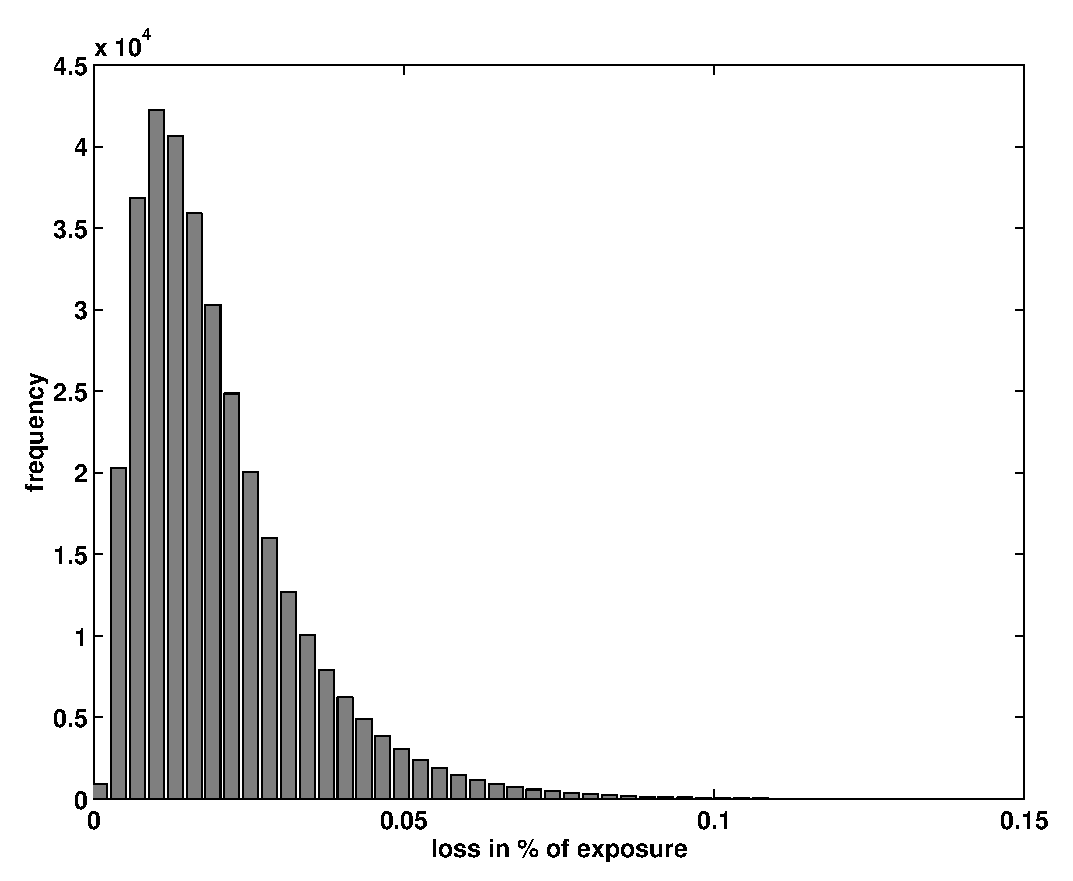
\includegraphics[angle=90,width=7cm,height=7cm,angle=-90]{chapters/chap_sample/figures/Histogram.eps}}
\subfigure[\label{f8b}]{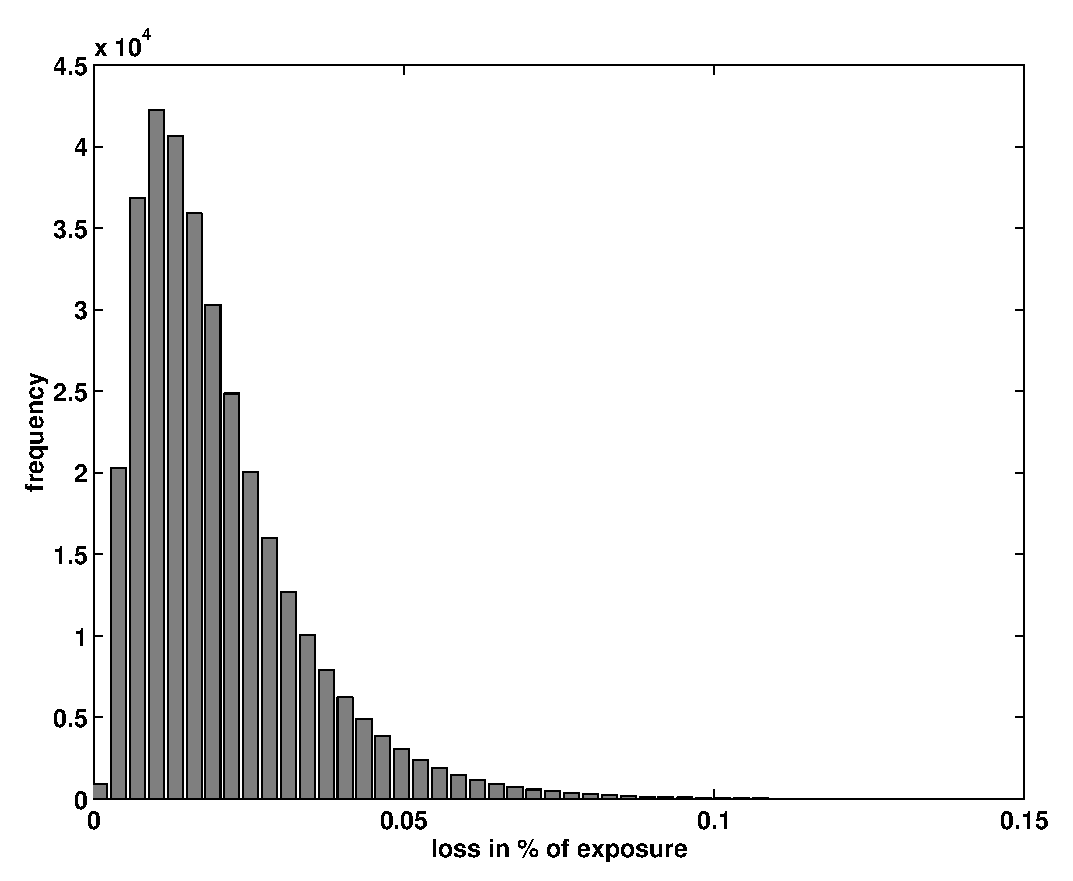
\includegraphics[angle=90,width=7cm,height=7cm,angle=-90]{chapters/chap_sample/figures/Histogram.eps}}
\end{center}
\caption[The bar charts depict the different risk contributions]{The bar charts depict the different risk contributions (top: 99\% quantile, bottom: 99.9\% quantile) of the business areas of a bank. The black bars
are based on a Var/Covar approach, the white ones correspond to shortfall risk.}
\end{figure}

\subsubsection{H3 A component part }
A component part for an electronic item is
manufactured at one of three \cite{mardia1979ma} different factories, and then delivered to
the main assembly line.Of the total number supplied, factory A supplies
50\%, factory B 30\%, and factory C 20\%. Of the components
manufactured at factory A, 1\% are faulty and the corresponding
proportions for factories B and C are 4\% and 2\% respectively. A
component is picked at random from the assembly line. What is the
probability that it is faulty? 

Some claim reengineering is too much "top down" in its orientation, planning and execution and, as a result, it fails
to fully consider all elements of the organizational system (such as customers or suppliers). By integrating
reengineering with Whole Systems change, using the Whole Organizational System approach, breakthrough results can be
achieved.

A fundamental notion \cite{yao2002can} is that of a\index{subspace}\index{vector 
space!subspace of} subspace of $F^n$. Let $V$ be a nonempty subset of 
$F^n$. Then $V$ is a {\it subspace} of $F^n$ provided $V$ is closed 
under vector addition and scalar multiplication, that is, 
\begin{enumerate} 
\item[\rm (a)] For all $u$ and $v$ in $V$, $u+v$ is 
also in $V$. 
\item[\rm (b)] For all $u$ in $V$ and $c$ in $F$, $cu$ is 
in $V$. 
\end{enumerate} 
Let $u$ be in the subspace $V$. Because $0u=0$, 
it follows that the zero vector is in $V$. Similarly, $-u$ is in $V$ 
for all $u$ in $V$. A simple example of a subspace of $F^n$ is the set 
of all vectors $(0,a_2,\ldots,a_n)$ with first coordinate equal to 0. 
The zero vector itself is a subspace.
\begin{itemize}
\item
It is the organization of work to achieve a result.
\item
It involves multiple steps and coordination of people and information.	
\begin{unnumlist}
\item
What data is available? 
\item
In what form do we have it?
\item
Who has it?
\end{unnumlist}
\item
It establishes management as the enabler and sustainer of process advantage.
\end{itemize}
The tool Process Mapping is used to help management and workers gain a fresh process insight. When applied to the
logistics process, it may help identify areas where breakthrough is possible. Traditional thinking about processes
comes from "process blindness."2 Because managers have not had to pay much attention to processes, this blindness has
plagued most companies for many years. A 1994 study that appeared in Information Week cited that on an operational
level, most senior managers have no idea how their companies operate. In other words, real day-to-day operational
performance is no longer understood, nor is it controlled on a real-time 
basis.\footnote{JIT II is a registered trademark of the BOSE Corporation and was developed by Lance Dixon.}

\begin{definition}\label{1def:linearcomb}
Let $u^{(1)},u^{(2)},\ldots,u^{(m)}$ be vectors in $F^n$, and let 
$c_1,c_2,\ldots,c_m$ be scalars. Then the vector
\[c_1u^{(1)}+c_2u^{(2)}+\cdots+c_mu^{(m)}\]
is called a {\it linear combination} \index{linear combination} of $u^{(1)},u^{(2)},\ldots,u^{(m)}$.
If $V$ is a subspace of $F^n$, then $V$ is closed under vector addition and 
scalar multiplication, and it follows easily by induction that a 
linear combination of vectors in $V$ is also a vector in $V$. Thus 
{\it subspaces 
are closed under linear combinations}; in fact, this can be taken as the 
defining property of subspaces.
The vectors $u^{(1)},u^{(2)},\ldots,u^{(m)}$ {\it span} $V$ \index{spanning set}
(equivalently, form a {\it spanning set} of $V$) provided every vector in 
$V$ 
is a linear combination of $u^{(1)},u^{(2)},\ldots,u^{(m)}$. The zero 
vector can be written as a linear combination of 
$u^{(1)},u^{(2)},\ldots,u^{(m)}$ with all scalars equal to 0; this is a 
{\it trivial linear combination}.\index{linear combination!trivial} The vectors
$u^{(1)},u^{(2)},\ldots,u^{(m)}$ are {\it linearly dependent} provided 
there are scalars $c_1,c_2,\ldots,c_m$, not all of which are zero, such 
that
\[c_1u^{(1)}+c_2u^{(2)}+\cdots+c_mu^{(m)}=0,\]
that is, the zero vector can be written as a {\it nontrivial linear \index{linear combination!nontrivial} 
combination} of $u^{(1)},u^{(2)},\ldots,u^{(m)}$.
\end{definition}


In addition to matrix addition, subtraction, and multiplication, there is 
one additional operation that we define now. It's perhaps the simplest of 
them all. Let $A=[a_{ij}]$ be an $m$ by $n$ matrix and let $c$ be a 
number \cite{hyvarinen2001ica}. Then the matrix $c\cdot A$, or simply $cA$, is the $m$ by $n$ 
matrix obtained by multiplying each entry of $A$ by $c$:
\[c A=[ca_{ij}].\]\index{matrix!scalar multiplication} \index{matrix!scalar multiple of}
The matrix $c A$ is called a {\it scalar multiple} of $A$.
\begin{VT1}

\VH{Think About It...}

Commonly thought of as the first modern computer, ENTAC was built in 1944. It took up more space than an 18-wheeler's
tractor trailer and weighed more than 17 Chevrolet Camaros. It consumed 140,000 watts of electricity while executing
up to 5,000 basic arithmetic operations per second. One of today's popular microprocessors, the 486, is built on a
tiny piece of silicon about the size of a dime.

\VT
With the continual expansion of capabilities, computing power will eventually exceed the capacity for human
comprehension or human control.

\VTA{The Information Revolution}{Business Week}
\end{VT1}
In order to break away from the traditional view where single functions dominate as a natural way of thinking, Keen
and Knapp pose several questions for management to answer:$^3$
\begin{enumerate}
\item
Who exactly is the customer or person to which the outcome.

\item
What must happen for the customer's request to be completely satisfied?
\begin{itemize}
\item
That change is so rapid that an organization needs increased face-to-face communication to make intelligent decisions.
\item
Successful strategies come from envisioning preferred futures.
\item
People will display more commitment to plans they help develop.
\end{itemize}
\item
	Who does the work and how does it come together?
\begin{enumerate}
\item 
That change is so rapid that an organization needs increased face-to-face communication to make intelligent
decisions.

\item
Successful strategies come from envisioning preferred futures.

\item	
People will display more commitment to plans they help develop.
\end{enumerate}
\item
Who does the work and how does it come together?
\end{enumerate}
\section{Glossary}
\begin{Glossary}
\item[360 Degree Review] Performance review that includes feedback from superiors, peers, subordinates, and clients.
\item[Abnormal Variation] Changes in process performance that cannot be accounted for by typical day-to-day variation. Also referred to as
non-random variation.
\item[Acceptable Quality Level (AQL)] The minimum number of parts that must comply with quality standards, usually stated as a percentage.
\item[Activity] The tasks performed to change inputs into outputs.
\item[Adaptable] An adaptable process is designed to maintain effectiveness and efficiency as requirements change. The process is
deemed adaptable when there is agreement among suppliers, owners, and customers that the process will meet
requirements throughout the strategic period.
\end{Glossary}


\chapterauthor{Dinesh Verma}{IBM}
\chapter{Introduction to AI}
\label{chap:intro:ai}

\lipsum[1-2]
\section{Introduction}\label{sec:intro:ai:intro}
\lipsum[2-4]

\section{Second Section}
\lipsum[2-4]

% \section{Glossary}
% \begin{Glossary}
% \item {xxx }
% \end{Glossary}
\chapter{Introduction to Sustainability}
\label{chap:intro:sustain}
\lipsum[1-2]
\section{Introduction}\label{sec:intro:sustain:intro}
\lipsum[2-4]
\chapter{Introduction to Emerging Markets}
\label{chap:intro:markets}

\lipsum[1-2]
\section{Introduction}\label{sec:intro:marketd:intro}
\lipsum[2-4]
\chapterauthor{Sourav Mazumder}{IBM}
\chapter{Challenges for AI and Sustainablity in Emerging Markets}
\label{chap:intro:final}

\lipsum[1-2]
\section{Introduction}\label{sec:final:ai:intro}
\lipsum[2-4]

\section{AI Governance in Emerging Markets}
\lipsum[2-4]

\section{Network Connectivity and Infrastructure Challenges}
\lipsum[2-4]

\section{Security Issues }
\lipsum[2-4]

\section{Data Considerations in Emerging Markets}
\lipsum[2-4]

\section{Reuse Considerations in Emerging Markets}
\lipsum[2-4]


\part{Addressing the Challenges}


\chapterauthor{Dinesh Verma}{IBM}
%\chapterauthor{Author Name2}{Affiliation text2}
% \chapterauthor{Author Name3}{Affiliation text3}
% \chapterauthor{Author Name4}{Affiliation text4}

\chapter{AI in the presence of limited connectivity}
\label{chap:limited_network}
%\lipsum[1-2]

This chapter looks at the challenges that arrives when AI/ML based solutions need to be deployed in an environment where the network connectivity is limited. A limited network is one where two communicating parties have limitations on exchanging data with each other. The limitation may arise due to the volume of data being too large compared to the throughput possible on the network, or due to the costs associated with transferring data,  or may be due to regulatory restrictions or security concerns. Regardless of the underlying cause, the basic challenge is that data can not be transferred across the network freely. 

\section{Introduction}
\label{sec:limited_network:intro}
% cover the following topics: 
% Workflow of AI (data collection, train model, inference) 

As mentioned in Chapter~\ref{chap:intro:ai}, an AI enabled system has two distinct stages in its life-cycle. The first stage deals with the creation of an AI model based on training data, and the second stage deals with the use of the AI model to make decisions on an operational piece of data. In both of these stages, limited network connectivity can pose a significant challenge in the effectiveness and operation of a solution. 

During the model creation stage, the key steps include collection of training data, cleaning and curation of the training data, and using the cleaned data to train an appropriate AI model. When the network is constrained, the task of collecting the data can become difficult. 

An alternative to moving the data is to move the training process past the point where the network is limited. However, if data was being collected from different training locations, this means different models trained at different locations need to be combined together. That requires specific mechanisms to handle the limitations. 

During the decision-making stage, operational data has to be used to make decisions. A limited network can make the movement of the operational data to the decision making location difficult. Compounding the challenge is the fact that the devices that may be presented closer to the location where data is being generated may have limited resources. 

\begin{figure}[htbp]
\centering
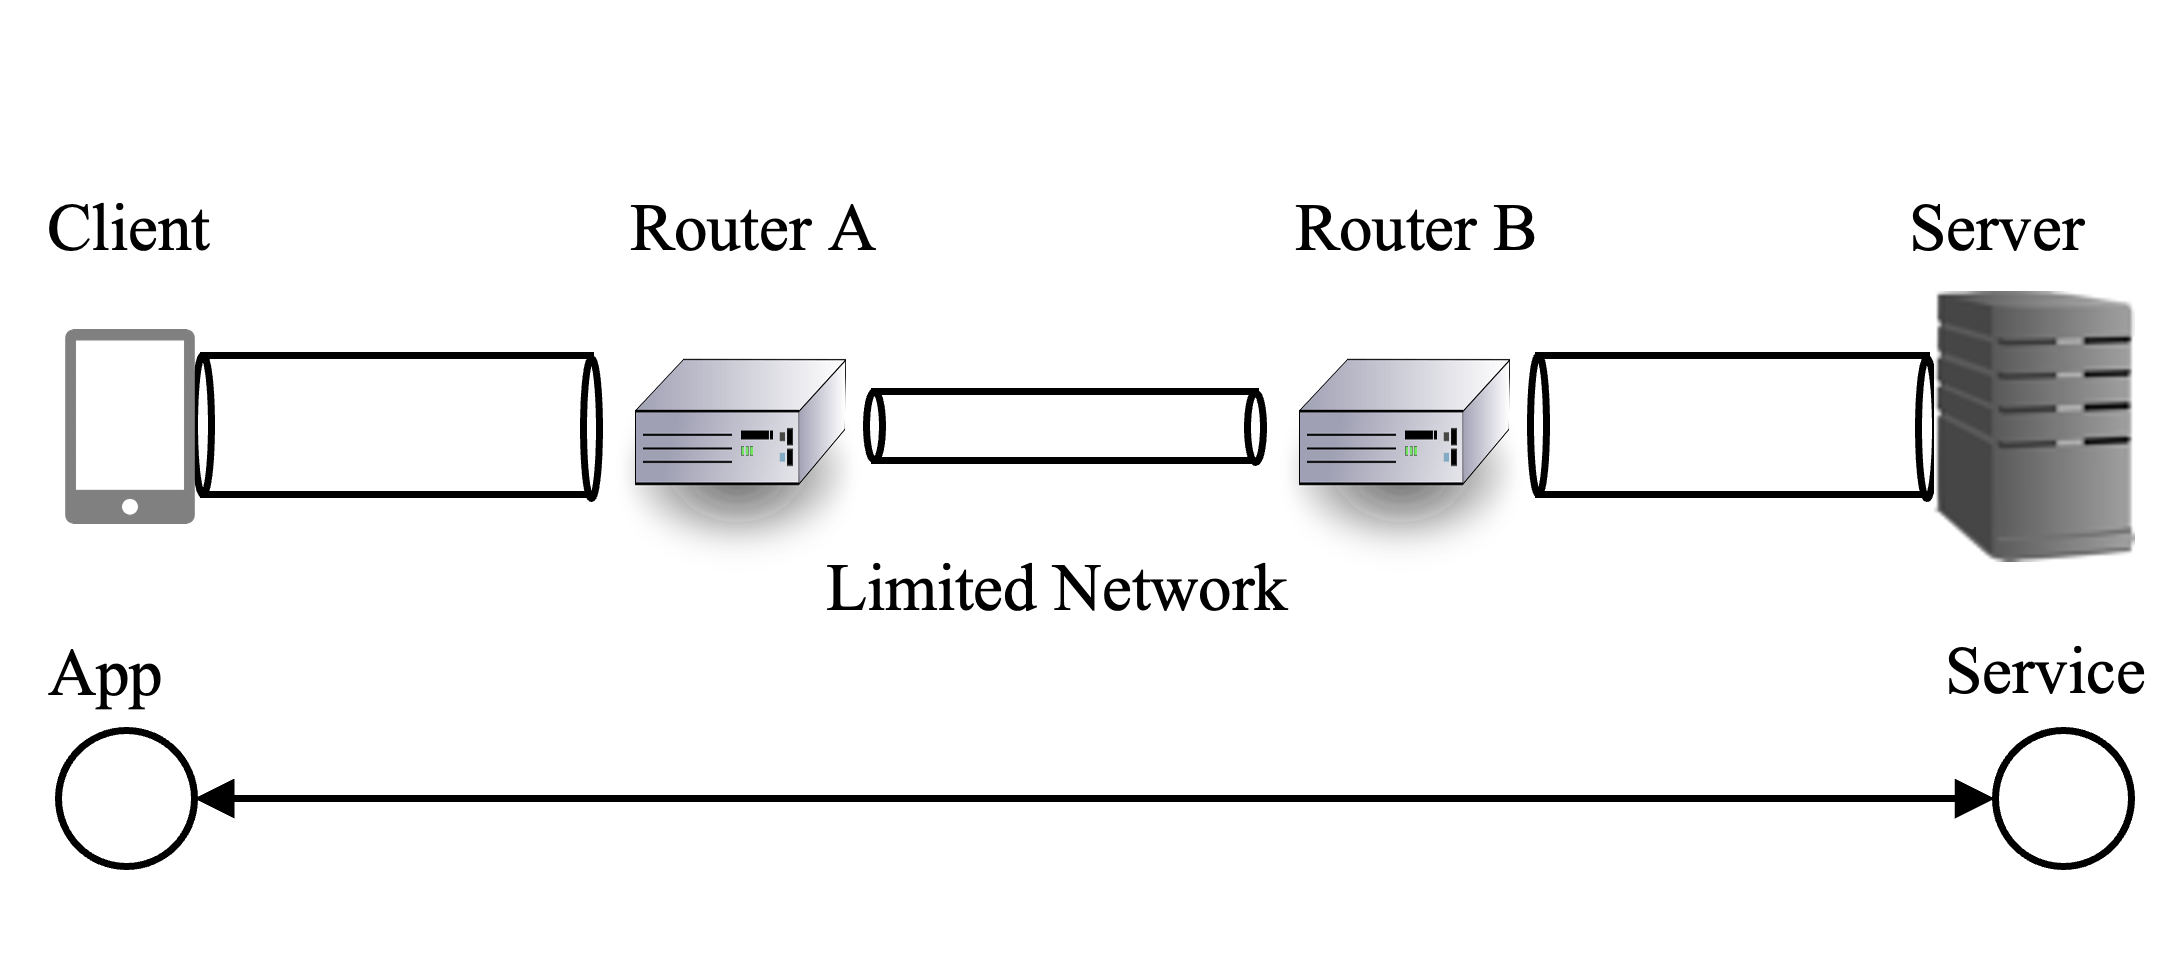
\includegraphics[height=2in] {chapters/chap_net_limited/chap_net_figures/fig1.png}
\caption{Abstracted Model of a Limited Network}
\label{fig:chap_net:ov}
\end{figure}

The challenge of data collection in a limited network environment can be illustrated using the simplified diagram shown in Figure~\ref{fig:chap_net:ov}. This figure shows a simplified model of a limited network. A client accesses a server through a network. Part of the network between the client and the server is constrained. The constrained network is flanked by two routers (A and B) which face the client and the server respectively. The network between the client and the router A and the network between the server and the router B are assumed not to be constrained. 

In these cases, an emerging economy would be on one side of the limited network and the services it wants to access would be on the other side. In other scenarios, the  client and the server may both be within an emerging nation, and the internal network in the nation could be constrained. 

When the application on the client needs to interact with a service on the server, the limited network would have an adverse impact of its performance and responsiveness. 

\section{Data Collection Challenges}
\label{sec:limited_network:collection}

During the task of data collection, we can assume that the client application shown in Figure~\ref{fig:chap_net:ov} is collecting information and sending it to the server shown in the same figure. The client may be a sensor, a microphone, a camera or applications on a phone that use the peripherals or devices within the phone. A phone can in some instances be used to record sounds, upload images and videos. 

The main task of the application on the client is to get the data generated locally successfully uploaded to the service. In order to do that in the presence of the limited network, the application needs to minimize the amount of data that is transferred over the constrained network. One approach to do such minimization is to compress the data flowing between the client and the server. 

This process is shown in Figure~\ref{fig:chap_net:compress}. A compression and a decompression function are introduced between the client and the server. The information from the client is compressed before it is sent over the limited network, and it is uncompressed after it leaves the limited network. 

The location of the compression function can be anywhere from the application (on the client device) to any (and including) device upto router A. Similarly, the location of the uncompression function can be anywhere between the server and router B. Since the networks between these segments are assumed to be fast without any constraints, the location would not have a material impact on the performance. 

When data is sent from the server to the client in the reverse direction, the tasks of compression and decompression needs to be performed in reverse location. However, since we are assuming that the data is primarily flowing from the client to the server, the compression is shown on the client side while the decompression is shown in the server side. In many sites, the site for compression and decompression would perform these operations for data flowing in both directions. 

\begin{figure}[htbp]
\centering
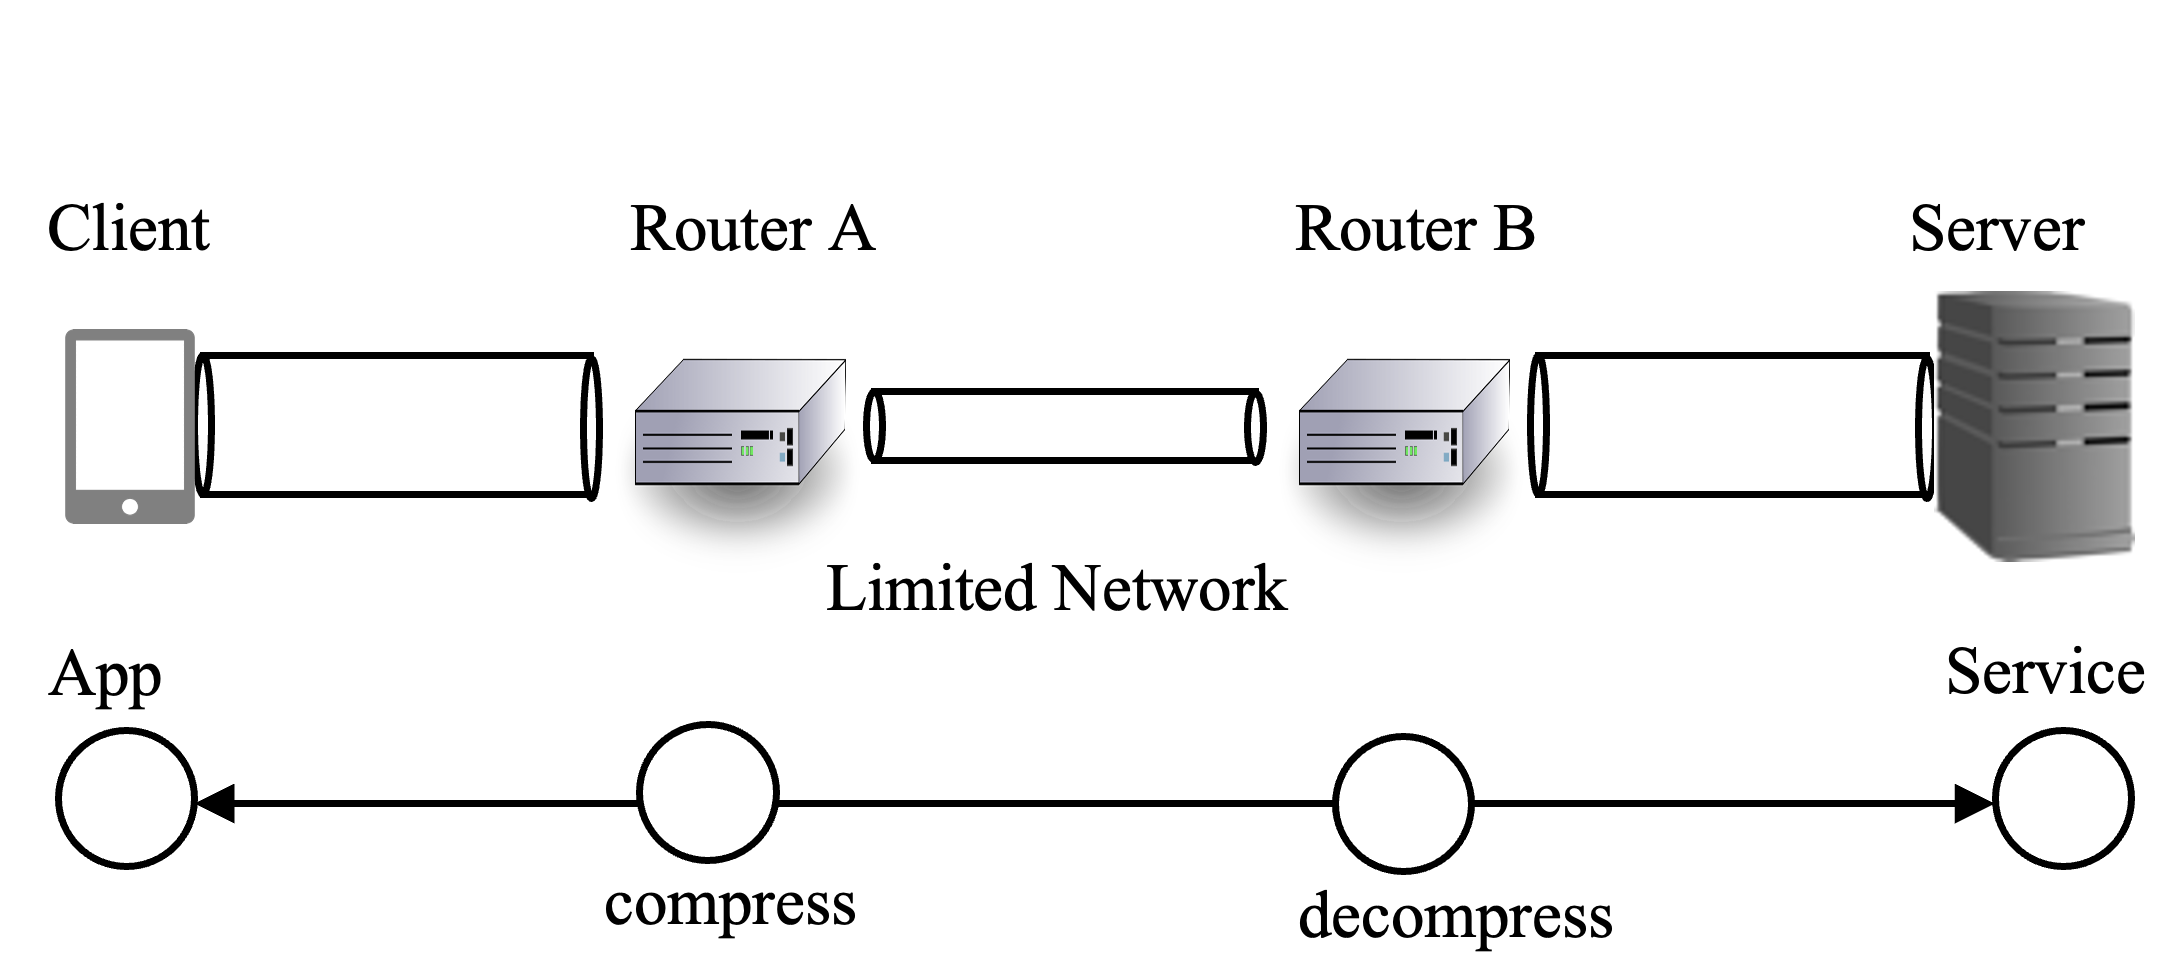
\includegraphics[height=2in] {chapters/chap_net_limited/chap_net_figures/fig2.png}
\caption{Compression to reduce data transfer}
\label{fig:chap_net:compress}
\end{figure}

There are many types of compression algorithms that can be used to reduce the amount of information flowing through a constrained network link.  Compression algorithms are classified into the two broad categories of lossless compression and lossy compression. In lossless compression, data is compressed so that the entire original data object can be reconstructed without any errors. In lossy compression, portions of the original data object are considered less important, and a better reduction is obtained by using approaches where those portions are discarded. Lossless compression is used for general data objects, while lossy compression is used for objects where some amount of loss can be tolerated, e.g. audio or video content where humans are able to make sense even if the content is slightly degraded. 

A commonly used set of lossless compression algorithms belong to the Lempel-Ziv family ~\cite{ziv1977universal, ziv1978compression}. These algorithms look for repeated patterns or sequences occurring in the content, and replace them with equivalent smaller representations on subsequent occurrences. The algorithm creates a table to store bit-patterns against the shorter representations. The table is generated dynamically depending on the contents of the object being compressed.

Lossy compression is usually more efficient than lossless compression. Some common standards, e.g. JPEG, MPEG and MP3 for audio/video use variations of lossy compression. In these schemes, the algorithm drop portions of the  data that is less important. See ~\cite{david2004data, sayood2017introduction} for a survey of both lossy and lossless data compression algorithms. 

One type of compression scheme is called byte-caching~\cite{le2012byte}, in which a dictionary is maintained between two devices with frequently occurring content replaced with a small  hash. Byte-cache builds the dictionary dynamically based on the contents of the packets  flowing between two pair of devices. The bytes that are to be matched with specific hash-codes are maintained in a cache at each of the devices, hence the name byte-cache. 

Byte caching relies on a shared dictionary to reduce size of data flowing between two devices. Other variations on dictionary based payload compression include maintaining multiple dictionaries at each point and selecting them on a packet by packet basis based on the content, or creating estimates for predicting future byte-streams based on current content, which may allow for more efficiency

If the network link is very constrained, e.g. a satellite link, one can deploy header compression~\cite{tye2003review} which tries to minimize the overhead in transmission of information. Standard headers protocols used for communication (e.g. in the Internet family of TCP/IP protocols) are designed for a general purpose network, and some of their fields may not be very useful under some special situations. Standards to compress headers are part of communication standards ~\cite{rfc1144, rfc2507, rfc3544}. Many of the fields in the packet header do not change frequently on some links. As an example, if a source and destination are communicating on a serial link, these two fields are going to remain the same regardless of the packet exchange. In these cases, one can use a streamlined header that does not require specifying these fields.

Some objects being transferred on the mobile network can be made available in different formats, with each format using a different amount of bandwidth on the network. Video streams, for example, can be encoded at different rates~\cite{pancha1994mpeg}. Many common types of video encoding schemes ~\cite{li2001overview} produce video that contains a base layer and several enhancement layers. The video quality is acceptable when only the base layer is sent to the receiver and becomes better as more and more enhancement layers are used. This allows a sender to control the data that a video stream consumes depending on the rate that is available.  


\begin{figure}[htbp]
\centering
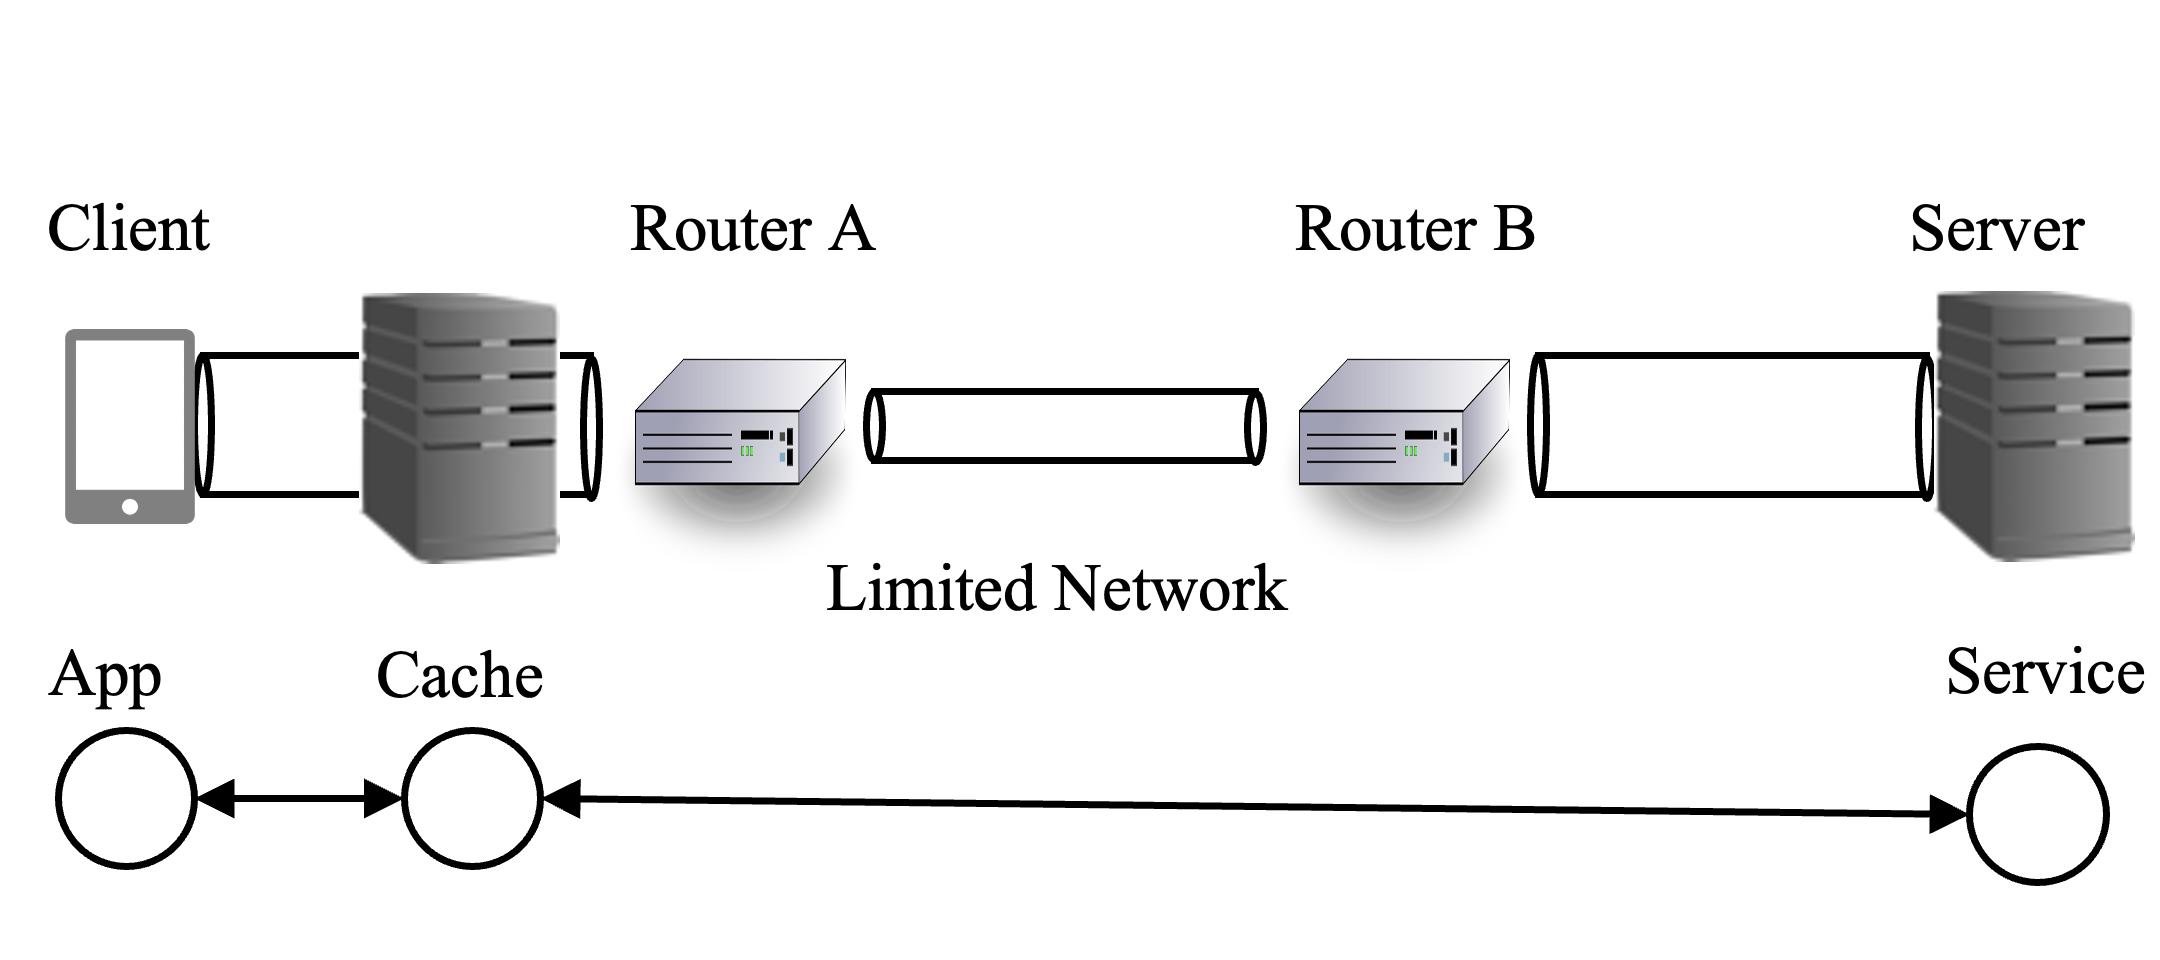
\includegraphics[height=2in] {chapters/chap_net_limited/chap_net_figures/fig3.png}
\caption{Caching to bypass data collection in a Limited Network}
\label{fig:chap_net:cache}
\end{figure}

In some cases, there may be many applications that may need to collect the same data source. For example, let us consider an emerging economy where several researchers are interested in training a machine learning model to understand the satellite imagery. In order to train the imagery, they can use imagery data that is available from various government agencies in US and Europe. If there are multiple users of the same data, it is possible to set up a caching service for the data in the nation itself. The caching service can retrieve the data once, and then let the other users obtain the data from the cache instead of obtaining it from the service across the constrained network. This setup is shown in Figure~\ref{fig:chap_net:cache}. 

While the caching approach works well in a technical sense, there may be some business issues which are hard to work around. If the different developers in the emerging economy belong to different companies, who should be the company running and operating the caching service? Is it appropriate for the caching service to redistribute content that belongs to some other entity -- one that holds the original data? The incentives to deploy a caching solution to reduce the bandwidth passed on the constrained link may not always be clear.   

Since we know the the data collection is meant for machine learning purposes, there are some other compression techniques that can also be used that are specific to machine learning. One such approach is the use of core-sets ~\cite{ mirzasoleiman2020coresets, lu2020robust}. When machine learning training data is collected, some of the training data may be redundant for the machine learning algorithm, in the same that it does not provide any additional new information that improves the model. The goal behind core-sets is to reduce the amount of data so that the quality of machine learning model is not compromised, but data points that do not improve the model are ignored. This provides an application-specific approach to compression. 

Another approach for reducing data compression is to only select data relevant for the machine learning task. As an example, suppose a data source is available on a well-connected portion of the Internet, e.g. satellite images may be available from the U.S. or European government agencies. A developer in an emerging economy wants to use those data sets to train machine learning models. The developer and the data source are separated by a trans-oceanic network which is expensive, high-latency and high-delay. It is worthwhile to note that all the data available in the US/European agency would not be relevant to the task of building a machine learning model in the emerging nation. As an example, the image data may cover all of the world, but the developer may want to train a model on the data collected for one country only. The developer could choose to use a computer located in US/Europe to download the whole data set, select the relevant parts of data of interest to the machine learning task, and only take that subset of data across the constrained link. This can cut down on the amount of data being transferred. 

\section{Model Training with limited networks}
\label{sec:limited_network:training}

% Moving model training to the edge (linear topology)
% data curation/labeling challenges
% federated learning (model iteration) 
% One-Shot federated learning 

\begin{figure}[htbp]
\centering
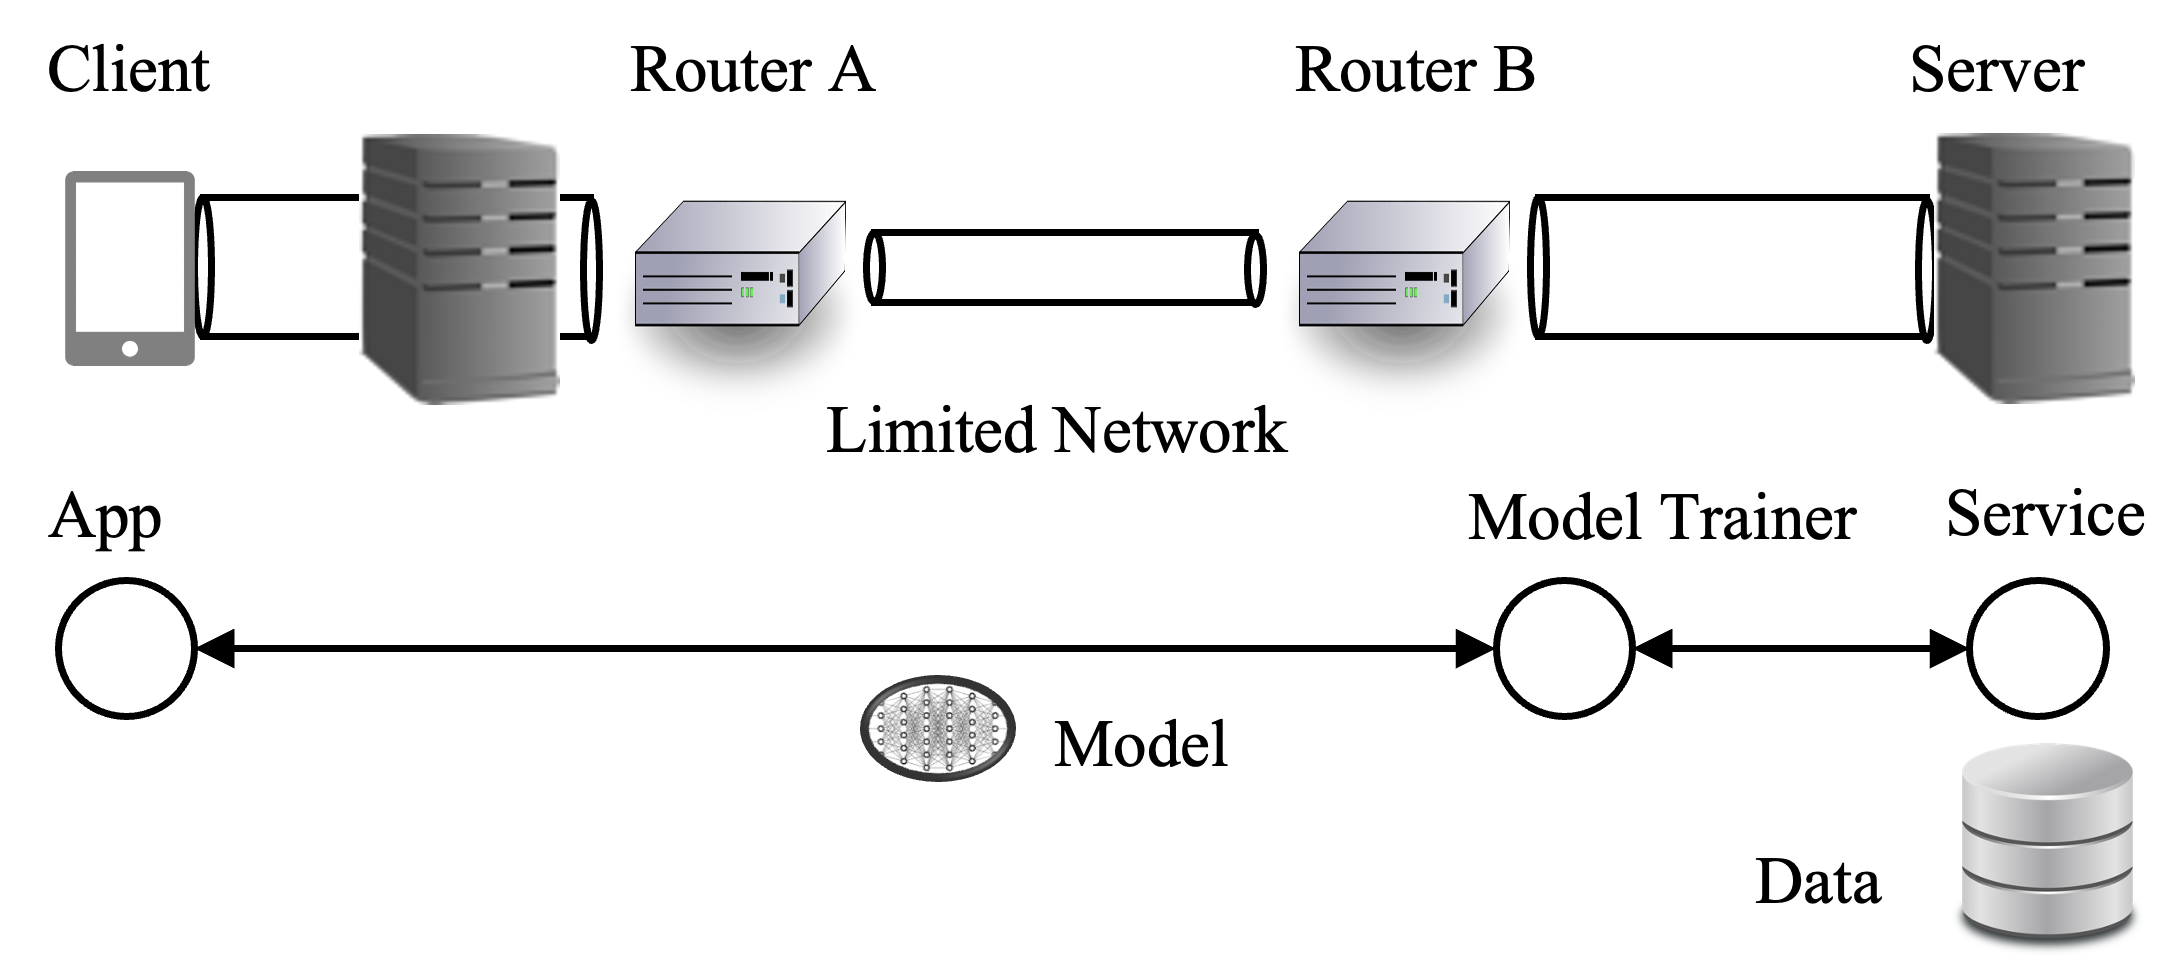
\includegraphics[height=2in] {chapters/chap_net_limited/chap_net_figures/fig4.png}
\caption{Learning past the Constrained Link}
\label{fig:chap_net:edge_learn}
\end{figure}


When model training needs to be done on a data source which is across a constrained network, another approach would be to avoid the constrained link altogether for data movement. If the model training process is moved over to the other side of the constrained link, one can only move the model across the constrained link. In general the model would be significantly smaller than the amount of data used to train it. 

This approach is shown in Figure~\ref{fig:chap_net:edge_learn}. Suppose data is present on the right-hand side of the system. Even though the client needing the data is present on the left-hand side, it is better to train an AI model on the right-hand side, and move the model instead of moving the data across the link. 

\begin{figure}[htbp]
\centering
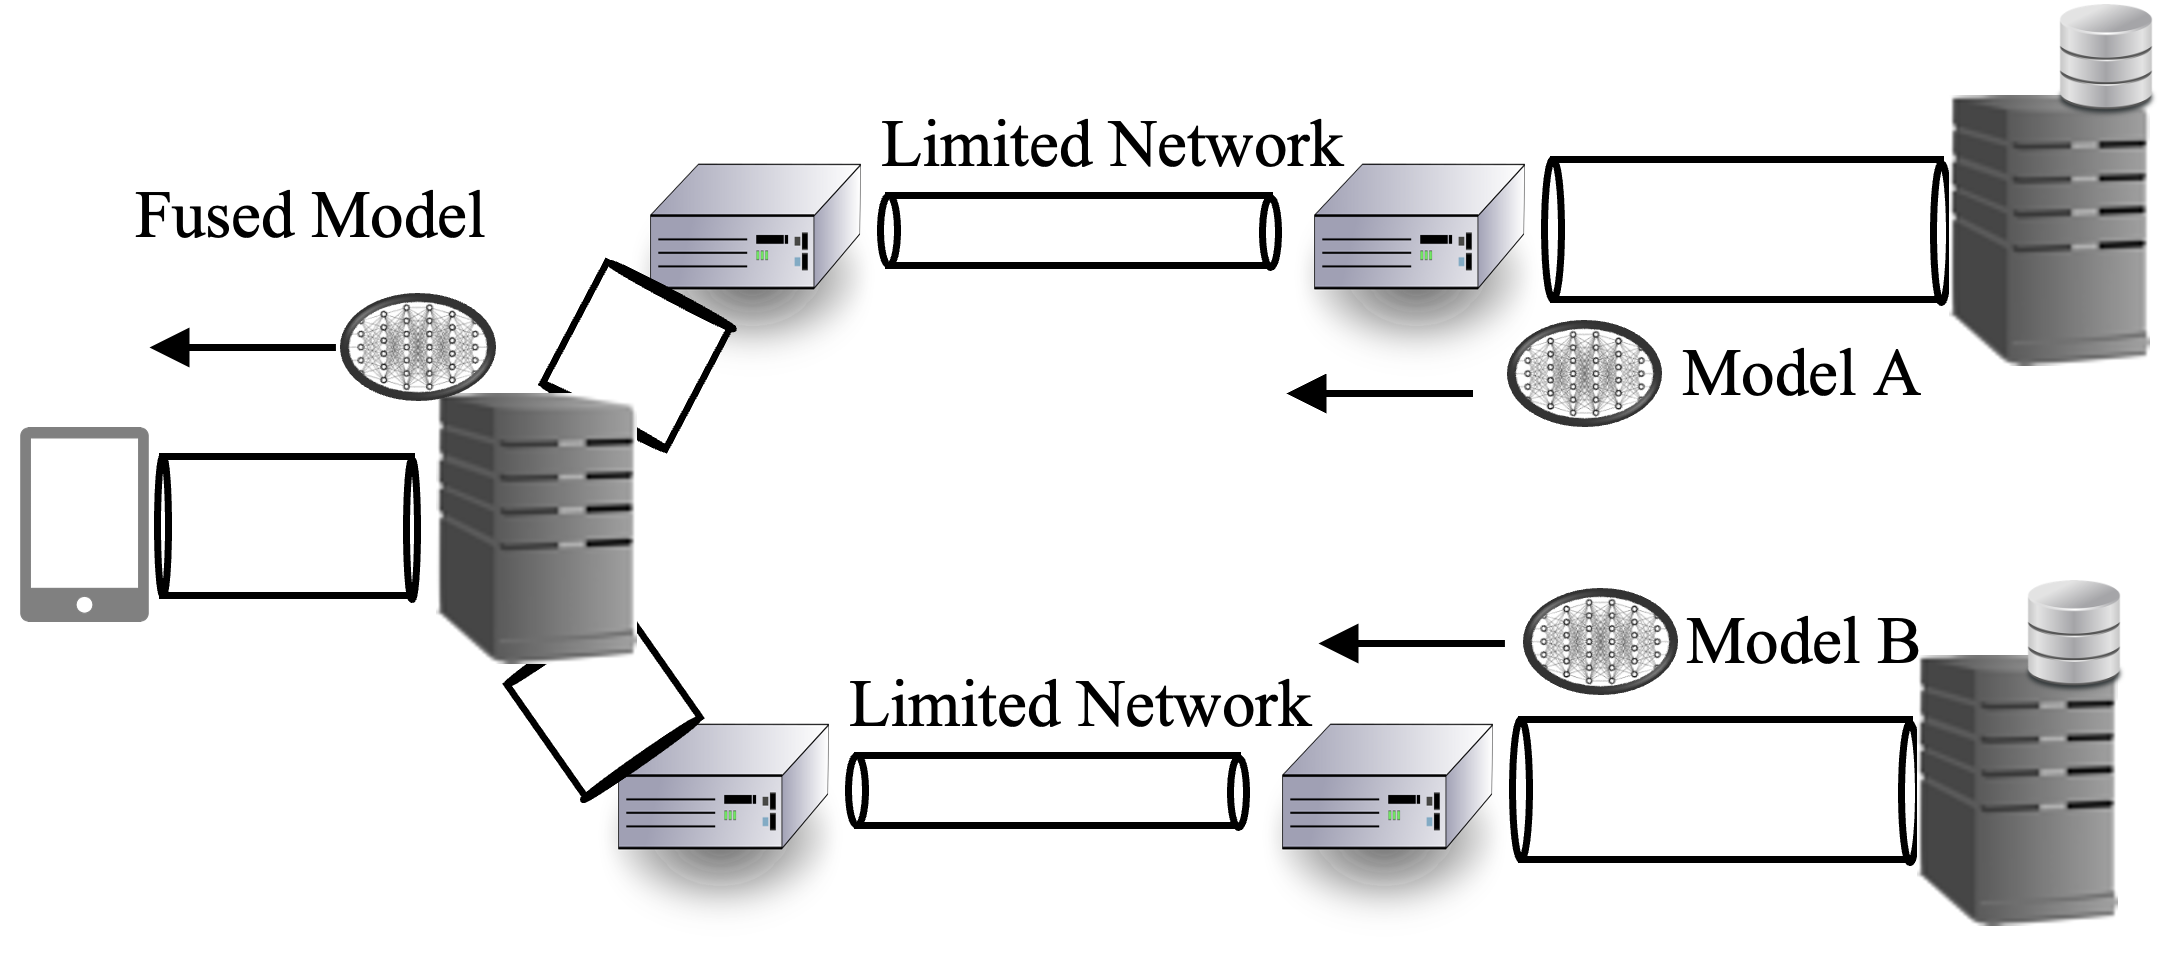
\includegraphics[height=2in] {chapters/chap_net_limited/chap_net_figures/fig5.png}
\caption{Federated Learning with a Limited Network}
\label{fig:chap_net:fedlearn}
\end{figure}

In some cases, the data may not be present at a single location but at many different locations. In some cases, the constraints on the data may be on accessing the different data sources. As an example, consider the situation of three different emerging nations, all of whom have data related to agricultural crops in their nations respectively. Ideally, they want to combine the data together. However, moving the data across the links may be too time-consuming. 

The techniques for federated learning~\cite{verma2021federated}
may be useful here. In Federated learning, each of the emerging nations can train their own models independently, and then the models are combined together into an aggregated combined model. Since the approach moves models over the constrained link, it works better than moving the data across. In using federated learning, an approach that minimizes the movement of models across the constrained links ~\cite{verma2022non} works better than those that move models multiple times. 

A sample scenario for federated learning is shown in Figure~\ref{fig:chap_net:fedlearn}. The figure takes the hypothetical situation where training data is present in two different locations, and each location has a limited network to the place where the model resulting from the training of the data is used, namely the client. The approach would be to have another server which is used to combine models trained by each of the locations with data. This setup can be useful for countries to share models with each other instead of sharing raw data with each other. 


\section{Inference with limited networks}
\label{sec:limited_network:inference}

% Three approaches 
% Compress data -- e.g. PCA or some other reduce representation 
% Move inference across the edge past the low latency 
% Move some layers to the edge, other layers at original site. 

% Make reference to the fact that optimization needs to be handled in the different stages. 
% Limited model - model optimization (chapter 2.2)




\chapter{AI in Presence of Limited Infrastructure}
\label{chap:limited_infra}

\lipsum[1-2]
\section{Introduction}\label{sec:limited_infra:intro}
\lipsum[2-4]
\paragraph{Neccessity is the Mother of Invention}
It is well known that the tight restrictions on poetry act as a forcing function for creativity.
The ecosystem of computing at the Edge is no different; limited bandwidth and limited computational resources force the designer and engineer to rethink a task, to formulate the process with minimal bandwidth, bit-depth, and dimensionality, e.g.~$\mbox{min}\left(\mbox{BBD}\right)$.
Under such constraints, one will likely find that reducing parameters in trained models, reducing the bit-depth and dimensionality of the in-coming raw data stream, and doing so in low-power system-on-chip solutions that are directly attached to the sensor, will elicit parsimonious solutions that will benefit from high generalizability as well as robustnes to concept drift.

\section{Goals}
\subsection{Information Density}
\paragraph{Optimize representations}
\subsection{Optimal Bandwidth Utilization}
\paragraph{Iteration with network measurements in training}
Reshuffle the hyperparameters iteratively 

\section{Benefits}
\subsection{Robustness}
\chapterauthor{Sheeba Prakash}{IBM}
\chapter {Data for AI}
\label{chap:data_for_ai}
\section{Introduction}\label{sec:data:intro}
\lipsum[2-4]

%Cover following topics

\section{Multiple Data Storage mediums and related challenges}
\label{sec:data:storage}
\lipsum[2-4]
Storage Medium -  Different storage medium and inconsistency of storing data

Sometime Hard copies 

Indigenous wisdom 

\section{How to link all data from various mediums together?}
\label{sec:data:link}
\lipsum[2-4]
Availability of tools to link all Data
Need for a tool to link all data wherever they reside, be it on cloud or on prem, or even hard copies is needed.

Availability of  Meta Data
Current data book keeping may not be  great. Not enough Meta data will be a common cause.



\section{Data Curation}
\label{sec:data:curation}
\lipsum[2-4]

We need curated data which will help an organization make good use of its data. It also helps to comply with  regulatory and security requirements.

Challenge in developing markets challenge would be to analyse and make meaning out of unstructured and unorganized data.  Effort needed to curate the data may be significant 

\section{Local Languages}
\label{sec:data:language}
\lipsum[2-4]

Language being different than English is another challenge. Tanzania -is an example. Multiple languages are spoken in this country.  Swahili and English being the most popular.   English that was inherited from colonial rule is widely spoken
reference - "https://en.wikipedia.org/wiki/Linguafranca". 
Swahali and English serve as working languages in the country, with Swahili being the official national language.
There are more speakers of Swahili than of English in Tanzania.
Wikipedia reference - 

reference -https://en.wikipedia.org/wiki/Tanzania

Core - technologies - not goood enough for handling
Huge challenge is finding the Common shared root ..  Even that does not 
Theology
Natural Language Does not rule out AI

\section{Data Scientists skills}
\label{sec:data:skills}
\lipsum[2-4]

Data Scientists - Skills may not be available-  

Can have alternate solutions here -
Nocode  may help build or Lowcode -  with minimum code
Crowd sourcing  - can be a good breeding platform that can also be Asset / Code reuse

Medical Repo - refer to webinar.- Doctor in rural area - Volunteers in that area - Project ecoh
Gives access to a larger set of expertise. or even distant experts. Having acces to these experts

- Countries around the globe- Doctors come in from various cpuntries get together.

%Tanzania - Bill Wright. - (will send across for reference)

Training/ Local Enablement - Locals trained - Community leaders. 
Community center/ church / where they come together. 
Centralized place where to go.

Water resource management for example - Adoption and usage. there are educated among Farmers and then also not so educated- 
Collectives- Leaders being educated and then they train local farmers..
Not online . rather in person. on the ground.
Adoption - How they adopt will be a good model.

\section{Capturing Indigenous Wisdom}
\label{sec:data:wisdom}
\lipsum[2-4]
\chapterauthor{Ryan Coffee }{Stanford}

How do we make sure Indigenous wisdom is not lost? 
Hoe to capture this?

\section{Challenges with applying best practices}
\label{sec:data:practice}
\lipsum[2-4]

Applying the best practices may be a challenge in emerging markets. Not enough supporting technology , skills among local citizens, 

Goal will be to come up with best practices.



\chapter{Security, Trust and Privacy of AI Solutions}
\label{chap:security_privacy}

\lipsum[1-2]
\section{Introduction}\label{sec:security_privacy:intro}


\section{Goals}\label{sec:security_privacy:goals}
\subsection{Obfuscation}
The rise of very large models with trillions ($10^{12}$) of parameters is sure to tax the energy production capacity in humanity.  
One of the least efficient parts of the AI ecosystem is the transfer of bits across networks for the sake of local aggregation for training. 
A key opportunity to alleviate such inefficiency lies in Federated Learning paradigms, but a security aspect for federated learning will expose critical systems to security risk. 
For this reason, data obfuscation for exchange on public network infrastructure would significantly reduce the exposure to security risk. 

\subsection{Provenance} 
Built on the authentication for key distribution of obfuscation schemes, the provenance of data 

\part{AI for Sustainability}

\chapter{AI enabled Solutions for Climate Change} 
\label{chap:climate_change}

\lipsum[1-2]


\section{Introduction to AI and Climate Change}\label{sec:climate_change:intro}
% Introduction to AI and Climate Change
% An in-depth look at the science behind climate change.
    % AI foundational model for climate
    % https://arxiv.org/pdf/2309.10808.pdf
    % Impact of climate event 
    
% AI in Renewable Energy
% Sustainable Agriculture Through AI
% Carbon Capture and Storage
  % Biodiversity credit system - few paragraphs
  % Adverse effects of tracking systems for animals - real world issues 
% Climate Prediction and Modeling
% Disasater warning syetem
    % widfire detection
    % monitoring of water bodies
% AI to validate climate change regulations
    % example/best practices reduce environmental impact - how can AI help

\lipsum[1-2]
\section{Second Section}
\lipsum[1-2]

\chapter{Water Management Solutions}
\label{chap:watermgmt}

\lipsum[1-2]
\section{Introduction}\label{sec:watermgmt:intro}
\lipsum[2-4]

%\part{Sustainability of AI}
%\include{chapters/ch1}


\bibliographystyle{plain}
\bibliography{bibtex_example}

\printindex
\cleardoublepage
\end{document}

